%%%%%%%%%%%%%%%%%%%%%%%%%%%%%%%%%%%%%%%%%%%%%%%%%%%%%%%%%%%%%%%%%%%%%%%%%%%%%%%
% Chapter 'Adsorption - CarbonDioxide - activated carbon Norit RB 1'
%%%%%%%%%%%%%%%%%%%%%%%%%%%%%%%%%%%%%%%%%%%%%%%%%%%%%%%%%%%%%%%%%%%%%%%%%%%%%%%
\subsection{Activated carbon Norit RB 1}
%
%%%%%%%%%%%%%%%%%%%%%%%%%%%%%%%%%%%%%%%%%%%%%%%%%%%%%%%%%%%%%%%%%%%%%%%%%%%%%%%
%%%%%%%%%%%%%%%%%%%%%%%%%%%%%%%%%%%%%%%%%%%%%%%%%%%%%%%%%%%%%%%%%%%%%%%%%%%%%%%
\subsubsection{Langmuir - ID 1}
%
\begin{tabular}[l]{|lp{11.5cm}|}
\hline
\addlinespace

\textbf{Sorbent:} & activated carbon \\
\textbf{Subtype:} & Norit RB 1 \\
\textbf{Refrigerant:} & CarbonDioxide \\
\textbf{Equation:} & Langmuir \\
\textbf{ID:} & 1 \\
\textbf{Reference:} & van der Vaart, Rick; HUISKES, CINDY; Bosch, Hans; Reith, Tom (2000): Single and Mixed Gas Adsorption Equilibria of Carbon Dioxide/Methane on Activated Carbon. In: Adsorption 6 (4), S. 311–323. DOI: 10.1023/A:1026560915422. \\
\textbf{Comment:} & None \\

\addlinespace
\hline
\end{tabular}
\newline

\textbf{Properties of sorbent:}
\newline
%
Property data of sorbent and subtype does not exist.

\textbf{Equation and parameters:}
\newline
%
Loading $w$ in $\si{\kilogram\per\kilogram}$ is calculated depending on pressure $p$ in $\si{\pascal}$ and temperature $T$ in $\si{\kelvin}$ by:
%
\begin{equation*}
\begin{split}
w &=& \frac{w_\mathrm{sat} K p}{1 + K p} & \quad\text{, and} \\
K &=& K_0 \exp \left( \frac{\Delta H}{R T} \right) & \quad\text{.}
\end{split}
\end{equation*}
%
The parameters of the equation are:
%
\begin{longtable}[l]{lll|lll}
\toprule
\addlinespace
\textbf{Par.} & \textbf{Unit} & \textbf{Value} &	\textbf{Par.} & \textbf{Unit} & \textbf{Value} \\
\addlinespace
\midrule
\endhead

\bottomrule
\endfoot
\bottomrule
\endlastfoot
\addlinespace

$\Delta H$ & $\si{\joule\per\mole}$ & 2.350000000e+04 & $w_\mathrm{sat}$ & $\si{\kilogram\per\kilogram}$ & 3.494354300e-01 \\
$K_0$ & $\si{\per\pascal}$ & 3.220000000e-10 & & & \\

\addlinespace\end{longtable}

\textbf{Validity:}
\newline
Equation is approximately valid for $50048.9 \si{\pascal} \leq p \leq 701434.0 \si{\pascal}$,  $294.5 \si{\kelvin} \leq T \leq 348.3 \si{\kelvin}$, and $0.0246555 \si{\kilogram\per\kilogram} \leq w \leq 0.282155 \si{\kilogram\per\kilogram}$.
\newline

\textbf{Visualization:}
%
\begin{figure}[!htp]
{\noindent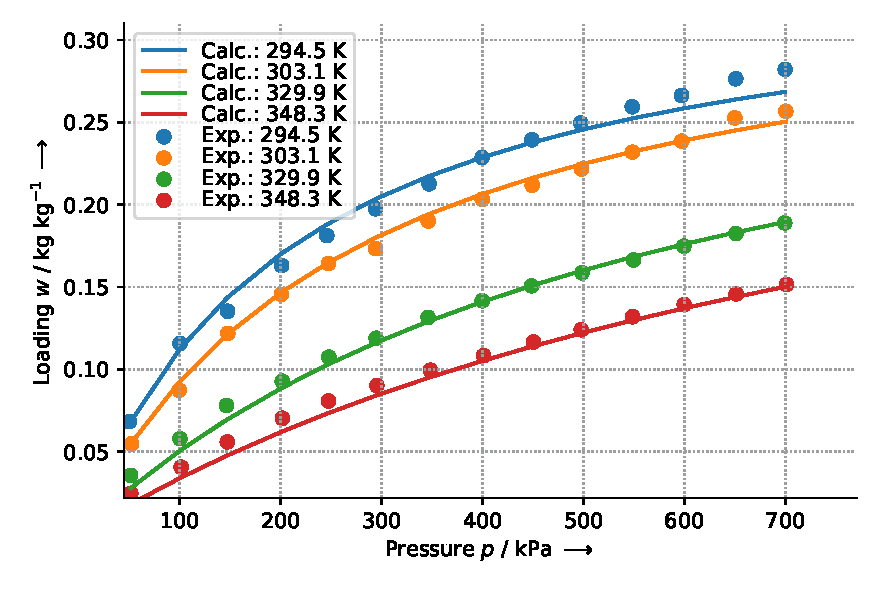
\includegraphics[height=10cm, keepaspectratio]{figs/ads/ads_CarbonDioxide_activated_carbon_Norit_RB_1_Langmuir_1.pdf}}
\end{figure}
%

To generate the figure, the following refrigerant functions were selected:
\begin{itemize}
\item Vapor pressure: VaporPressure\_EoS1 - ID 1
\item Saturated liquid density: SaturatedLiquidDensity\_EoS1 - ID 1
\end{itemize}

The uncertainity of the experimental data is:
\begin{itemize}
\item Data source $\,\to\,$ Data was taken from table
\end{itemize}

The mean absolute percentage error (MAPE) between the experimental and calculated data results in 4.06\%.
\FloatBarrier
\newpage
%%%%%%%%%%%%%%%%%%%%%%%%%%%%%%%%%%%%%%%%%%%%%%%%%%%%%%%%%%%%%%%%%%%%%%%%%%%%%%%
